\chapter{Accurate Soft Error Simulation Using Partitioning} \label{ch3}

As process technology continues to the scale down, the likelihood of a radiation induced error increases. This trend provides a need for accurate and efficient methods to calculate the soft error rate of a given circuit. Since it is expensive and time consuming to design a circuit and test at a later time, efficient tools that can accurately determine the error rate for a given netlist before fabrication can significantly reduce the design time. However, it has proven to be very difficult to characterize combinational circuits due to three pulse masking factors. The masking factors are as follows:

\begin{enumerate}
	\item Logical Masking: The pulse is removed due to the boolean inputs on the gate during pulse generation or a controlling value on an off-input during pulse propagation.
	
	\item Electrical Masking: The first order RLC effects within the gate cause the pulse to degrade and fully attenuate.
	
	\item Temporal Masking: The pulse arrives at a flip-flop but does not meet the set-up and hold time parameters. 
\end{enumerate}

Considering the above factors, all current soft error simulators consist of modeling a particle at a specific energy, which is used in an equation to model the error pulse shape \cite{injeq}. Once the pulse is generated, it is propagated through the combinational logic to the output. It is then assumed that the output is connected to a flip-flop thus the set-up and hold times are considered. It has been shown in \cite{MARS_C,METSys} that concurrent estimation of all masking factors is required in order to ensure that the soft error rate is calculated accurately. However, due to limitations on simulation time and available memory, efficient and accurate consideration of all masking factors has proven to be a difficult and ongoing problem. 

There have been many approaches to improve the estimation of the three masking factors. The most common method to calculate the logical masking effect is the use of a Monte Carlo based simulation which consists of randomly applying patterns as in \cite{Accurate_Masking,SERA,SEMM,PARAM_DESC,SETA_LA}. While this approach is very easy to implement, it suffers from accuracy and run time issues when the circuit has more than 30 inputs. In the case of large circuits, the simulator must resort to generating random input patterns which cover only a small subspace of the possible inputs. This implies that the error in logical masking estimation increases with the circuit size. 

To enhance Monte Carlo based simulation, the authors in \cite{PTM} propose the use of probabilistic transfer matrices (PTM). This approach consists of representing the Boolean functions within a matrix in which Boolean operations can be applied. While being exact in the estimation of the probability, the use of PTMs are not ideal since they have high memory and simulation time costs which do not scale to large circuits. The authors in \cite{Han2014} propose an enhanced alternative to the PTM method which uses stochastic logic to calculate the signal probabilities for logical masking estimation. While their method is fast, it relies on the use of random input patterns that can limit the accuracy of the calculation.

Another common approach found in \cite{Chen2013,Li2016} uses the correlation coefficient method (CCM) proposed in \cite{Ercolani1989}. This method uses basic gate signal probability functions to determine the output. For example, the probability of an AND gate is given as $P(O) = P(A)P(B)$ where $P(O)$ is the output probability, $P(A)$ is the probability of input $A$ being ``1" and $P(B)$ is the probability of inputs $B$ being ``1". A drawback with using the basic probability functions is that they are unable to consider the correlations between signals. CCM improves on this by adding a correlation factor to estimate the signal probability. While CCM does provide quick estimation of the logical masking effects with virtually no memory overhead, it can only estimate first order correlation. This implies that as the circuit gets larger, the accuracy of the method substantially decreases.

The last approach discussed in this section, which is of most concern in this paper, is the use of binary decision diagrams (BDDs). BDDs provide an accurate way to determine the logical masking effects since they are a condensed canonical form of a Boolean function. The main problem with BDDs however, is that they scale exponentially with circuit size thus increasing the difficulty in modeling medium to large circuits. Despite this problem, there have been many proposed simulators that use BDDs \cite{FASER,MARS_C,METSys}. The main advantage to the use of BDDs is that all input patterns can be considered concurrently thus allowing for exact calculation of logical masking probabilities.

To alleviate the inherent blow up problem, the authors in \cite{FASER} propose the use of partitioning. In their work, they show that the use of partitioning allows for much faster calculation of the soft error rate with no threat of blowup at a cost of accuracy. The authors in \cite{METSys} also investigate partitioning but do not give an in depth study on how partitioning effects the output error. In both approaches, the circuit is partitioned before simulation with each partition size being set to a predetermined value. In this section, a new tool is proposed that uses partitioning to reduce the simulation time. Furthermore, compared to existing approaches, the new tool allows for the integration of an accurate electrical masking model that can calculate the output pulse shape for any input pulse. This implies that the pulse width will not be approximated as an integer value. The methods in \cite{METSys} and \cite{FASER} use algebraic decision diagram (ADDs) and multi-terminal BDDs (MTBDD) which have terminating nodes representing a pulse with a calculated width or magnitude. To reduce complexity, these simulators consider pulses with similar width or magnitude using the same terminating node and modify the decision diagram structure accordingly so that the cases are merged. However, when an accurate masking model is used, the width and magnitude has a smaller granularity decreasing the likelihood of pulses having the same width leading to a reduction in merged cases. This implies that nearly every propagated pulse will require a new output terminal leading to blowup in the decision diagram size and complexity. 

In addition to \cite{FASER} and \cite{METSys}, the authors in \cite{Gangadhar2008} propose a simulation tool which discretized the simulation time into time steps which are used for analysis throughout the circuit. As proposed, the approach uses integer values to propagate a square shaped pulse thus reducing the number of required time steps and providing fast simulation times. However, as stated before, the use of accurate electrical masking models necessitates the use of finer time steps so that the accuracy is preserved. If accurate models are used in \cite{Gangadhar2008}, the simulation time is immense due to a large number of time steps.

The proposed simulator has the capability of considering multiple concurrent pulse strikes commonly referred to as multiple event transients (METs). The consideration of multiple strikes has become a concern due to smaller feature sizes, leading to a lower critical charge for upset, and the closer placement of transistors \cite{Rossi2005}. These type of events can occur in two forms: single event multiple transient (SEMT) and multiple event multiple transient (MEMT). A SEMT is defined as the case where a single radiation particle upsets multiple transistors causing multiple transients pulses. A MEMT is defined as when multiple particles hit different circuit components simultaneously. While the probability of the SEMT vs the MEMT depends strongly on the radiation environment, methods developed for one type of error can easily be modified to consider the other. 

There are a few existing methods that include the consideration of multiple event errors. The authors in \cite{METSys} consider the correlation of METs however their method uses BDDs which tend to blow up and uses the width and amplitude to consider the pulse shape. While they do investigate the use of partitioning, their method is only tested for small circuits using only a few concurrent pulses. An additional simulation tool used for MET analysis found in \cite{Fazeli2011} uses probabilistic functions. This approach has shown to be fast and efficient but is not suited for the use of complicated electrical masking methods. To improve on the existing methods, the simulator FAST\_MET (Fast and Accurate Simulation Tool for Multiple Event Transients) which uses BDDs to calculate the logical maksing effect in conjunction with the accurate pulse approximation tool proposed. FAST\_MET improves on the method in \cite{METSys} by allowing for the integration of accurate electrical masking models and through the extensive use and evaluation of partitioning to avoid BDD blow up.    

\section{Preliminaries} \label{ch3:prelim}

A crucial aspect in the estimation of the logical masking effects is accurate creation of the Boolean functions. To ensure full consideration of the logical masking effects, Boolean functions must be created to evaluate the circuit inputs for pulse generation and the off-inputs for pulse propagation.

When a high energy particle strikes a transistor, the magnitude and polarity of the pulse will depend on the configuration of the transistor. In the case of CMOS logic, a transient pulse is generated when a particle hits a blocking transistor. This will, in turn cause the transistor to temporarily conduct current allowing for the generation of the voltage pulse. In Fig. \ref{NANDS} a 2 input NAND gate is given to demonstrate this mechanism. In the NAND gate, a particle can hit a single PMOS or a NMOS transistor to cause an error. However, since the transistor must be blocking, the input pattern of the gate has a large effect on where the error will occur and the polarity of the pulse. 

For example, in the 2 input NAND gate in Fig. \ref{NANDS}, if both inputs have a value of ``1", a strike on either of the PMOS transistors will likely cause a transient pulse. In the case of one input having a ``0" value and the other a ``1" value,  a strike on the blocking NMOS transistor will cause an error. In the case of both inputs having a ``1" value, the gate will only generate a transient pulse if both NMOS transistors are struck concurrently. Addition, the polarity of the pulse also requires consideration. If the output is has a ``1" value, the pulse will start at a high value, go low and back to a high value. When the output has a ``0" the pulse will start at a low value, go high and back to a low value. Based on this observation, the function for the pulse generation for the AND, NAND, OR and NOR are given in Table \ref{table:gentable} for a $N$ number of inputs with each $i$-th input denoted as $I_i$.

\begin{figure}[!htbp]
	\centering
	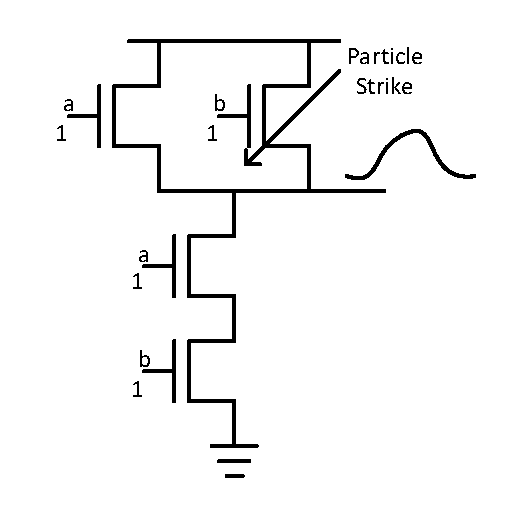
\includegraphics[width=0.5\linewidth]{Figures/NAND_Strike}
	%where an .eps filename suffix will be assumed under latex, 
	%and a .pdf suffix will be assumed for pdflatex; or what has been declared
	%via \DeclareGraphicsExtensions.
	\caption{A low-high-low transient pulse being generated by a strike on the PMOS.}
	\label{NANDS}
\end{figure}

\begin{table}[ht]
	\begin{center}
		\caption{Functions for Transient Pulse Generation}
		\label{table:gentable}
		\begin{tabular}{|c|c|c|}
			\hline
			Gate & Polarity & Generation Function ($F(G)$) \\ 
			\hline
			AND & Rising & $F(G) =  \lnot (I_1 \land I_2 \land ... I_N)$ \\
			\hline
			AND & Falling & $F(G) = I_1 \land I_2 \land ... I_N$ \\
			\hline
			NAND & Rising & $F(G) = I_1 \land I_2 \land ... I_N$ \\
			\hline
			NAND & Falling & $F(G) = \lnot (I_1 \land I_2 \land ... I_N)$ \\
			\hline
			OR & Rising & $F(G) = \bar{I_1} \land \bar{I_2} \land ... \bar{I_N}$ \\
			\hline
			OR & Falling & $F(G) = \lnot ( \bar{I_1} \land \bar{I_2} \land ... \bar{I_N})$ \\
			\hline
			NOR & Rising & $F(G) = \lnot ( \bar{I_1} \land \bar{I_2} \land ... \bar{I_N})$ \\
			\hline
			NOR & Falling & $F(G) = \bar{I_1} \land \bar{I_2} \land ... \bar{I_N}$ \\
			\hline
		\end{tabular}
	\end{center}
\end{table}

For the consideration of the generation of METs, the equations in Table \ref{table:gentable} must be modified such that the joint probability of the error occurring is considered. In the case of pulse generation, it is assumed that a single radiation particle will strike two or more gates causing transient pulses. As stated previously, in order for a pulse with a specific polarity to be generated, the output of the gate must have a specific value. Based on this, the probability of pulses being generated ($P_{gen}$) assuming it strikes $N$ gates with sufficient energy is given in equation \ref{pul_gen} where $P(G_{i,p})$ is the probability that gate $G_i$ is capable of generating a pulse of polarity $p$. If the pulse generated is rising, $G_{i,p}$ pertains to the probability that the output of $G_{i,p}$ is ``0". If the pulse is falling, $G_{i,p}$ is the probability of the output being ``1".

\begin{equation} \label{pul_gen}
P_{gen} = \prod_{i=1}^{N} P(G_{i, p})
\end{equation}

A particle hitting two transistors simultaneously allows for multiple cases since the input may be such that the struck gate is not blocking. Based on this, the total number of possible ways a strike can produce a pulse ($P_{num}$) is given in equation \ref{num_eq} assuming a $N$ number of struck gates and $r$ as the number of gates that produce a transient pulse.

\begin{equation} \label{num_eq}
P_{num} = 2*\sum_{r=1}^{N} \frac{N!}{(N-r)!}
\end{equation}

Equation \ref{num_eq} is based on the fact that multiple pulses are not always generated when a particle strikes both transistors. As stated previously, the polarity and existence of the pulse depends on the input patterns. If one assumes that the particle hits a $N$ number of gates, this creates a $P_{num}$ number of cases where $P(C_i)$ represents the probability of case $i$ calculated using equation \ref{pul_gen}. The total probability of the inputs having the values to generate a SET or MET ($P_{gen}$) is given below:

\begin{equation} \label{err_eq}
P_{gen} = \sum_{i=1}^{P_{num}} P(C_i)
\end{equation}

In the case of a pulse being propagated to the input of gate, the pulse will be masked if one of the off-inputs has a controlling value. Fig. \ref{Prop_NAND} gives a NAND gate with one of the inputs having a pulse and the other input having a controlling ``0" value. In this case, the output will be a logical ``1" value despite the pulse on the input.

\begin{figure}[!htbp]
	\centering
	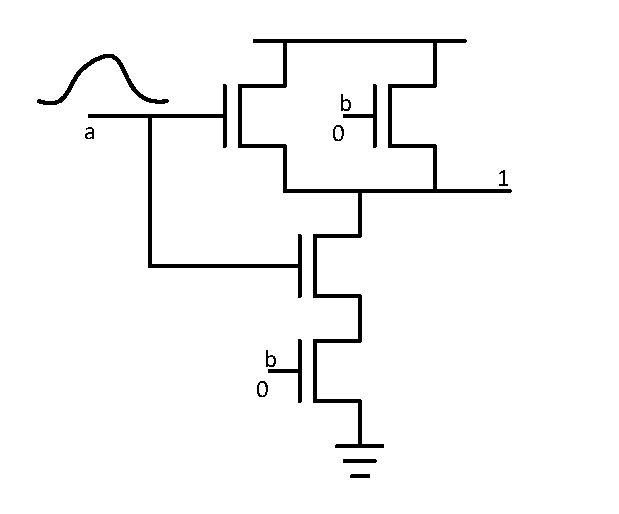
\includegraphics[width=0.55\linewidth]{Figures/Prop_func}
	%where an .eps filename suffix will be assumed under latex, 
	%and a .pdf suffix will be assumed for pdflatex; or what has been declared
	%via \DeclareGraphicsExtensions.
	\caption{A transient pulse being masking by a controlling value on the off-input.}
	\label{Prop_NAND}
\end{figure}

To calculate the logical masking factor during pulse propagation, the functions of the off-inputs are calculated using the logical AND operation. Assume that $F(OI_i)$ is the Boolean function of the off-input $OI_i$ representing the input patterns that allow a non-controlling value and there are a $N$ number of inputs, the function representing the case where the pulse is propagated ($F(M)$) is given below:

\begin{equation} \label{prop_eq}
F(M) = F(OI_1) \land F(OI_2) \land ... F(OI_N)
\end{equation}

\noindent In equation \ref{prop_eq} only $N-1$ inputs are considered since the input which contains the transient pulse is not included in the calculation. 

For the consideration of METs, two or more pulses may arrive at a gate. If the two pulse case is assumed, there are three possible ways that the pulses can be propagated: the pulse on $a$ is propagated and $b$ is masked, the pulse on $b$ is propagated and $a$ is masked and, lastly, both pulses are propagated simultaneously providing an output pulse. Fig. \ref{Prop_MET} provides an illustration of the cases.

\begin{figure}[!htbp]
	\centering
	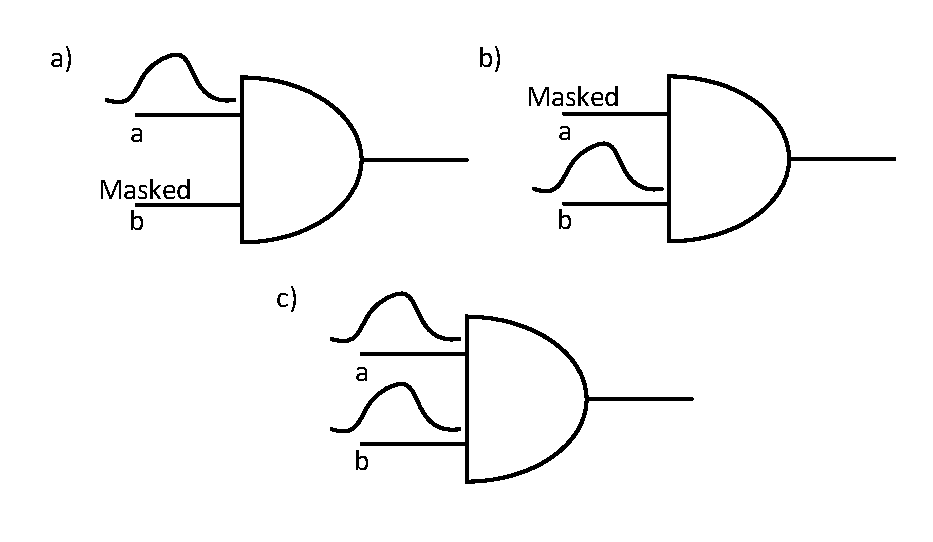
\includegraphics[width=0.80\linewidth]{Figures/Prop_MET}
	%where an .eps filename suffix will be assumed under latex, 
	%and a .pdf suffix will be assumed for pdflatex; or what has been declared
	%via \DeclareGraphicsExtensions.
	\caption{(a) A transient pulse arriving on input a and masked on b. (b) A pulse arriving on input b and masked on a. (c) Two pulses arriving on the inputs simultaneously.}
	\label{Prop_MET}
\end{figure}

Table \ref{table:prop_table} gives the propagation functions $F(G)$ for each case with $F(a_p)$ and $F(b_p)$ being the functions representing the input values that allow for the pulse to be propagated. While this example is only for a two input gate, larger gates can be considered similarly.

\begin{table}[ht]
	\begin{center}
		\caption{Functions for a MET Arriving on the Inputs of a NAND Gate}
		\label{table:prop_table}
		\begin{tabular}{|c|c|}
			\hline
			Case & Propagation Function ($F(G)$) \\ 
			\hline
			a & $F(G) = F(a_p) \land \lnot F(b_p)$ \\
			\hline
			b & $F(G) = \lnot F(a_p) \land F(b_p)$ \\
			\hline
			c & $F(G) = F(a_p) \land F(b_p)$ \\
			\hline
		\end{tabular}
	\end{center}
\end{table}

Based off equation \ref{num_eq}, the total number of cases can be calculated as the number of combinations assuming $i = 1,2,...N$ simultaneous pulses. Assuming that $P_{num}$ is the number of possible cases and $r_i$ represents a $i$ number of concurrent pulses, the equation for the total number of propagation cases is given below:

\begin{equation} \label{prop_num}
P_{num} = \sum_{i=1}^{N} \frac{N!}{(N-r_i)!}
\end{equation} 

Based on equation \ref{prop_num}, the total probability at a gate $G$ ($P(G_{tot})$) with the assumption that $P(G_i)$ is the probability of pulse $i$ arriving at gate $G$ is given below:

\begin{equation} \label{tot_gate}
P(G_{tot}) = \sum_{i}^{P_{num}} P(G_i)
\end{equation}

When a SET or MET is generated, it is represented as an event $E_k$ with $k$ being the event number. For each event, the generated transients are propagated through gates to the primary outputs. Once the pulse arrive at the gate output, the temporal masking probability can be considered. Based off the equation found in \cite{Omana_Trap}, let  $P_{L,i}$ be the probability of the pulse being latch on primary output $i$, $W$ be the pulse width, $t_{setutp}$ and $t_{hold}$ being the setup and hold times respectively and $T_{clk}$ be the clock period, the probability of a pulse being latch on an output flip-flop is calculated in the below equation:

\begin{equation} \label{temp_eq}
P_{L,i} = \frac{W - (t_{setup} + t_{hold})}{T_{clk}}
\end{equation}

Assuming that the pulses from event $E_k$ propagate to a $M$ number of primary outputs with each output having a probability of $P_{L,i}$ the probability of error for event $E_k$ is calculated as the following:  

\begin{equation} \label{event_eq}
P(E_k) = \sum_{i=1}^{M} P_{L,i}
\end{equation}

To evaluate the error probability for all events, the mean error susceptibility (MES), defined in \cite{METSys} is used. The MES represents the average probability of error for all events combined. Assuming that there are a $n_E$ number of events and $n_d$ number of input probability distributions, the MES is found using the following equation:

\begin{equation} \label{MES}
MES = \sum_{k=1}^{n_E} \frac{P(E_k)}{n_E n_d}
\end{equation}

Based off the MES, the soft error rate ($SER$) can be calculated as in below where $R_{eff}$ represents the effective concentration of particle in the given area, $P_{eff}$ is the probability of a particle hitting the sensitive region of a transistor and $A$ as the area of the sensitive volumes.

\begin{equation} \label{SER}
SER = MES*R_{eff}*P_{eff}*A 
\end{equation}

\section{Description of the FAST\_MET Simulator} \label{ch3:desc}

FAST\_MET is a fast and accurate tool to estimate the soft error rate. The method aims to provide a good trade-off between simulation time and accurate SER calculation. To accurately determine the logical masking effects, BDDs are used. A BDD is a tree structure which can be used to represent a Boolean function. The first instance of the use of BDDs for function representation was proposed in \cite{Bryant1986} and has continued to be used regularly in circuit simulation and synthesis since. Fig. \ref{BDD_AND} gives the representation of a AND gate as BDD. Note that the structure consists of nodes which represent variables. For each node, there are two branches, one denoting a ``true" value (solid line) and the other a ``false" value (dashed line). The BDD graph also consists of multiple paths to two terminating nodes, one with a ``true" value denoted by ``1" and one with a ``false" value denoted by ``0".

\begin{figure}[!htbp]
	\centering
	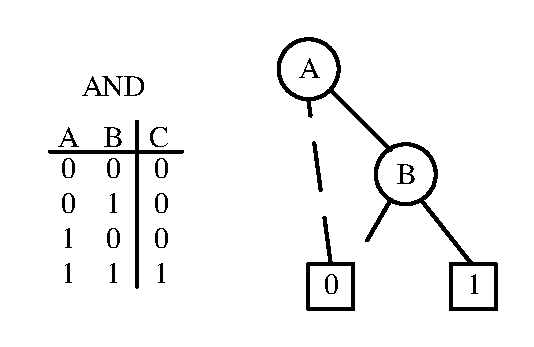
\includegraphics[width=0.55\linewidth]{Figures/BDDFunc}
	%where an .eps filename suffix will be assumed under latex, 
	%and a .pdf suffix will be assumed for pdflatex; or what has been declared
	%via \DeclareGraphicsExtensions.
	\caption{The truth table and corresponding BDD for an AND gate.}
	\label{BDD_AND}
\end{figure}

The main advantage of a BDD is that they provide an efficient canonical form to represent a Boolean function. Specifically, this means that Boolean operations (such as AND, NAND, OR ... etc) can be easily and quickly applied to the graph. In the case of the FAST\_MET simulator, BDD representation of the functions are used to both calculate the signal probability and the probability for pulse propagation.

In FAST\_MET, the goal is to accurately and efficiently represent a ``sensitization function" as a BDD. A sensitization function is defined as the Boolean function that allows for a generated transient pulse to propagate through a circuit. Once the function is derived, it can be evaluated to determine the logical masking probability of a pulse.

In addition to BDDs, the FAST\_MET simulator operates in a topological order. This implies that the primary inputs will be visited first. For each primary input visited, it is represented as a variable in a BDD. Once all inputs are visited, the simulator starts on the gates within the circuit. When a gate is visited, the sensitization function representing the gate output is calculated. The ``1" terminal on this BDD represents the Boolean function that makes the output a ``1" value. To increase efficiency, the FAST\_MET simulator also generates a rising and falling pulse at each gate using the method proposed in Chapter \ref{ch2} for a specific energy.

When a pulse is generated, the gate input functions are considered using the input sensitization functions. If the pulse is rising (starting from a low value then going high), the pulse is only generated when the output is low. To consider this, the BDD function is inverted such that a termination to ``1" represents the case at which the pulse exists. Similarly, if the pulse is falling, the output must be a high value. Since the function already denotes a high value on the output, the sensitization function can be used directly. Additionally, as discussed in Section \ref{ch3:prelim}, in the case of a gate having multiple inputs, the output function must be considered according to Table \ref{table:gentable}. Using the table, the correct generation function can be found by applying the function for the gate specified. Fig. \ref{BDD_GEN} provides an example of the creation of the generation functions for a gate.

\begin{figure}[!htbp]
	\centering
	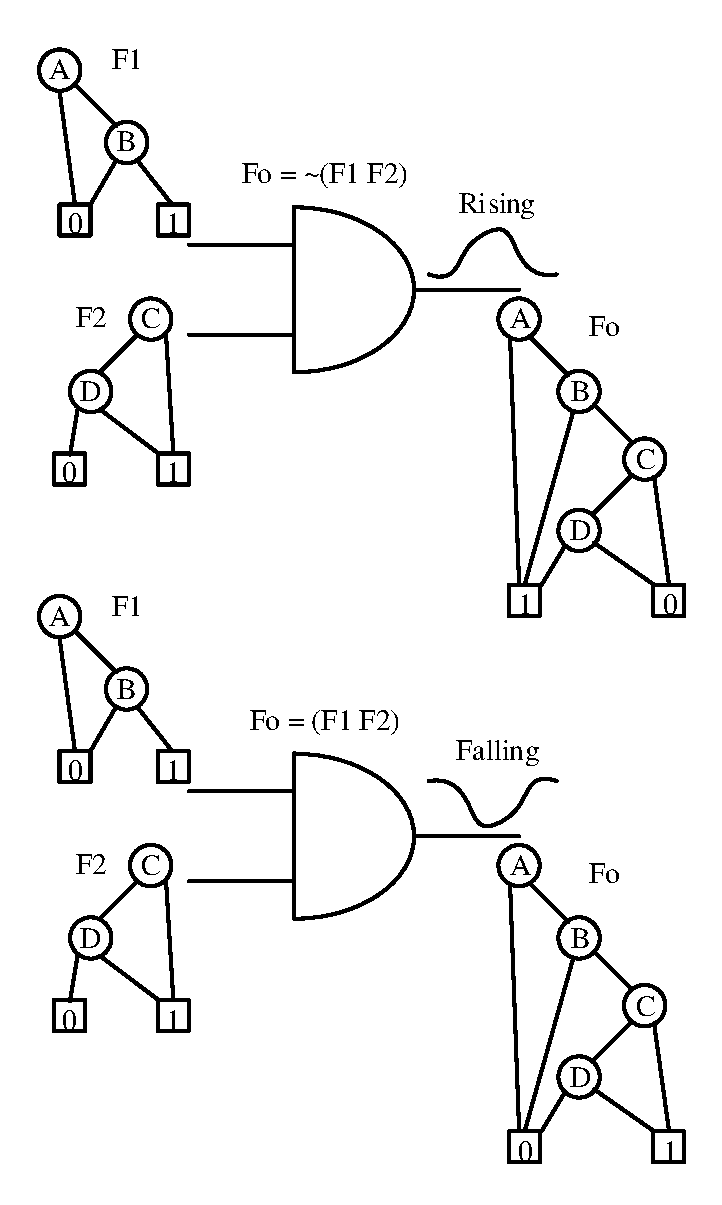
\includegraphics[width=0.65\linewidth]{Figures/gen_func}
	%where an .eps filename suffix will be assumed under latex, 
	%and a .pdf suffix will be assumed for pdflatex; or what has been declared
	%via \DeclareGraphicsExtensions.
	\caption{An example of the BDD creation for a rising and falling pulse.}
	\label{BDD_GEN}
\end{figure}

To consider the MET case, the location and correlation between the pulses must be considered. As discussed in \cite{Ebrahimi2016}, layout information is important in accurately modeling the location of the MET for a real design since gates that are near each other in a netlist may not necessarily be close in the layout. In this section, for the sake of simplicity, METs are generated using close proximity nodes from the netlist. Just for simple comparison and analysis, using the netlist is not problematic. 

To determine the logical masking effects of a MET, the correlation between the inputs of both struck gates are found by using the logical AND operation between the generation functions derived as in Table \ref{table:gentable}. The logic behind this operation is that all pulses must be logically sensitized concurrently. Since the functions may share common inputs, they may have dependencies that must be considered. 

In the case of pulse propagation, the sensitization functions are represented as BDDs. As discussed in Section \ref{ch3:prelim}, a pulse will propagate through a gate if all off-inputs have a non-controlling value. As can be observed in equation \ref{prop_eq}, the functions representing the case at which the off-input has a non-controlling value are logically AND'd together. The basis behind this idea is that all off-inputs must be non-controlling in order for the pulse to be propagated. 

To consider pulse propagation in the FAST\_MET simulator, the logic functions are first represented in a BDD. A logic function is the Boolean function which provides the variable states that allow a ``1" and a ``0" value. The sensitization function for the gate is then determined by using the logical AND operation on each off-input BDD. If the non-controlling value for the gate is a ``0", such as in a OR gate, the BDDs are inverted so that the ``1" terminal represents the case at which the pulse propagates. If the non-controlling value is a ``1" the BDDs are left unchanged. The result of this operation is a single BDD in which the paths that lead to the ``1" terminal represent all of the input patterns that allow the pulse to propagated while the paths that lead to the ``0" terminal represent the patterns that will mask the pulse.

In the case of multiple pulses arriving at a gate simultaneously referred to a convergent pulses, the off-inputs are considered as discussed previously. As shown in Table \ref{table:prop_table}, a MET can result in multiple output cases which must be considered. The first case is where only one pulse will propagate, which is calculated as previously discussed. All remaining cases include the circumstances where multiple pulses will arrive at the gate input simultaneously. In these cases, the logic function is determined by using the AND operation on the input functions which have a pulse. The resulting function from this operation is then AND'd with the non-controlling off-input logic functions. The basis behind this idea is that the pulse sensitization functions give the cases where a pulse will arrive at the gate input. For example if two pulses arrive simultaneously, both pulses must be sensitized concurrently. The logical AND states that both functions must evaluate to true indicating that the pulse arrives at the inputs while all off-inputs must be non-controlling for the pulse to be propagated.

\section{FAST\_MET Simulation Flow}

The goal of the FAST\_MET simulator is to calculate the SER of a circuit. To do this, the simulator must inject pulses in each gate. The main difficulty for this type of simulation is that for even relatively small circuits, it may take an intractable amount of simulation time and memory to consider all generation and propagation cases. The FAST\_MET simulator provides a good trade off compared to existing methods since it uses the pulse approximation method in Chapter \ref{ch2} in conjunction with BDDs to accurately and quickly determine the SER.

The first step for the FAST\_MET simulator is to partition the circuit. As shown in \cite{FASER,METSys}, the use of BDD functions can lead to memory blowup. To alleviate this issue, FAST\_MET partitions the circuit into a user defined number of parts. It is shown in Section \ref{ch3:results} that the use of partitioning can substantially reduce the simulation time at a cost of accuracy in the SER estimation. For this work, the circuits were partitioned using the Fiduccia and Mattheyses (FM) algorithm \cite{Fiduccia1982} which allows for a circuit to be partitioned into two parts in linear time. To achieve a $k$-part partition, the FM algorithm can be applied recursively a k-1 number of times. This algorithm was chosen based off its linear time complexity and relatively easy integration into the FAST\_MET tool. While the FM algorithm was used in this work, other partitioning tools such as hMetis \cite{hMetis} can be used. Partitioning the circuit improves performance by reducing the size of the logic and pulse sensitization BDDs. For moderately large circuits or larger, partitioning must be used since the BDD functions increase exponentially in size with respect to the number of inputs.

After partitioning, the FAST\_MET simulator processes the primary inputs of the circuit. At each input node, the signal probability is set and the BDD variables are initialized such that each input is a variable. In this work, it is assumed that there are no pulses on the inputs. However, if the method is used for the consideration of sequential circuits such as in \cite{MiskovZivanov2007}, pulses can be injected on the inputs. This is due to the inputs being connected to the output of a flip-flop which drives the circuit.

After the inputs are processed, the internal nodes are visited in a topological order. At each node, at least one pulse is injected for a given charge. The particle effect is modeled as a current pulse using equation \ref{qeq}. A current source is placed on the output of the gate to simulate the particle effect and the resulting pulse shape is determined using the method discussed in Chapter \ref{ch2}. Multiple pulses can be injected concurrently in a gate, however the simulation time and memory resources increase substantially as more pulses are injected.

Additionally, FAST\_MET is able to simulate the effects of a MET. To accommodate METs, each injected pulse or MET is given an event number $k$ to create an event $E_k$. This is important since FAST\_MET injects pulses at each gate concurrently to speed up the SER characterization. Thus, when an MET is generated, a pulse is created on two or more gates which all have the same event number.

Once the pulses are injected and the corresponding BDD functions are determined, FAST\_MET propagates all pulses found on the gate inputs. Each fanin gate is checked individually for pulses. If a pulse is found, the propagation function is determined as in Section \ref{ch3:desc}. If the function evaluates to a false value, implying that there are no input patterns that allow the pulse to be propagated, the pulse is not considered further. However, if the function is not false, the output pulse shape is calculated. This operation continues for each pulse found on the inputs. 

When a node is on the edge of a partition circuit, the values calculated on the previous partition must be considered. To do this, each node on the output edge of a partition is evaluated to determine their probability. This value is stored with the pulse which is propagated between the partitions. Since a partition may be separated from the primary inputs that drive it, virtual inputs are created which contain all pulses with their attached probabilities from the respective gate in the previous partition. Using these values, the probabilities are multiplied by the evaluated probability function to determine the overall probability. This is demonstrated in Fig. \ref{PART_PROP}.

\begin{figure}[!htbp]
	\centering
	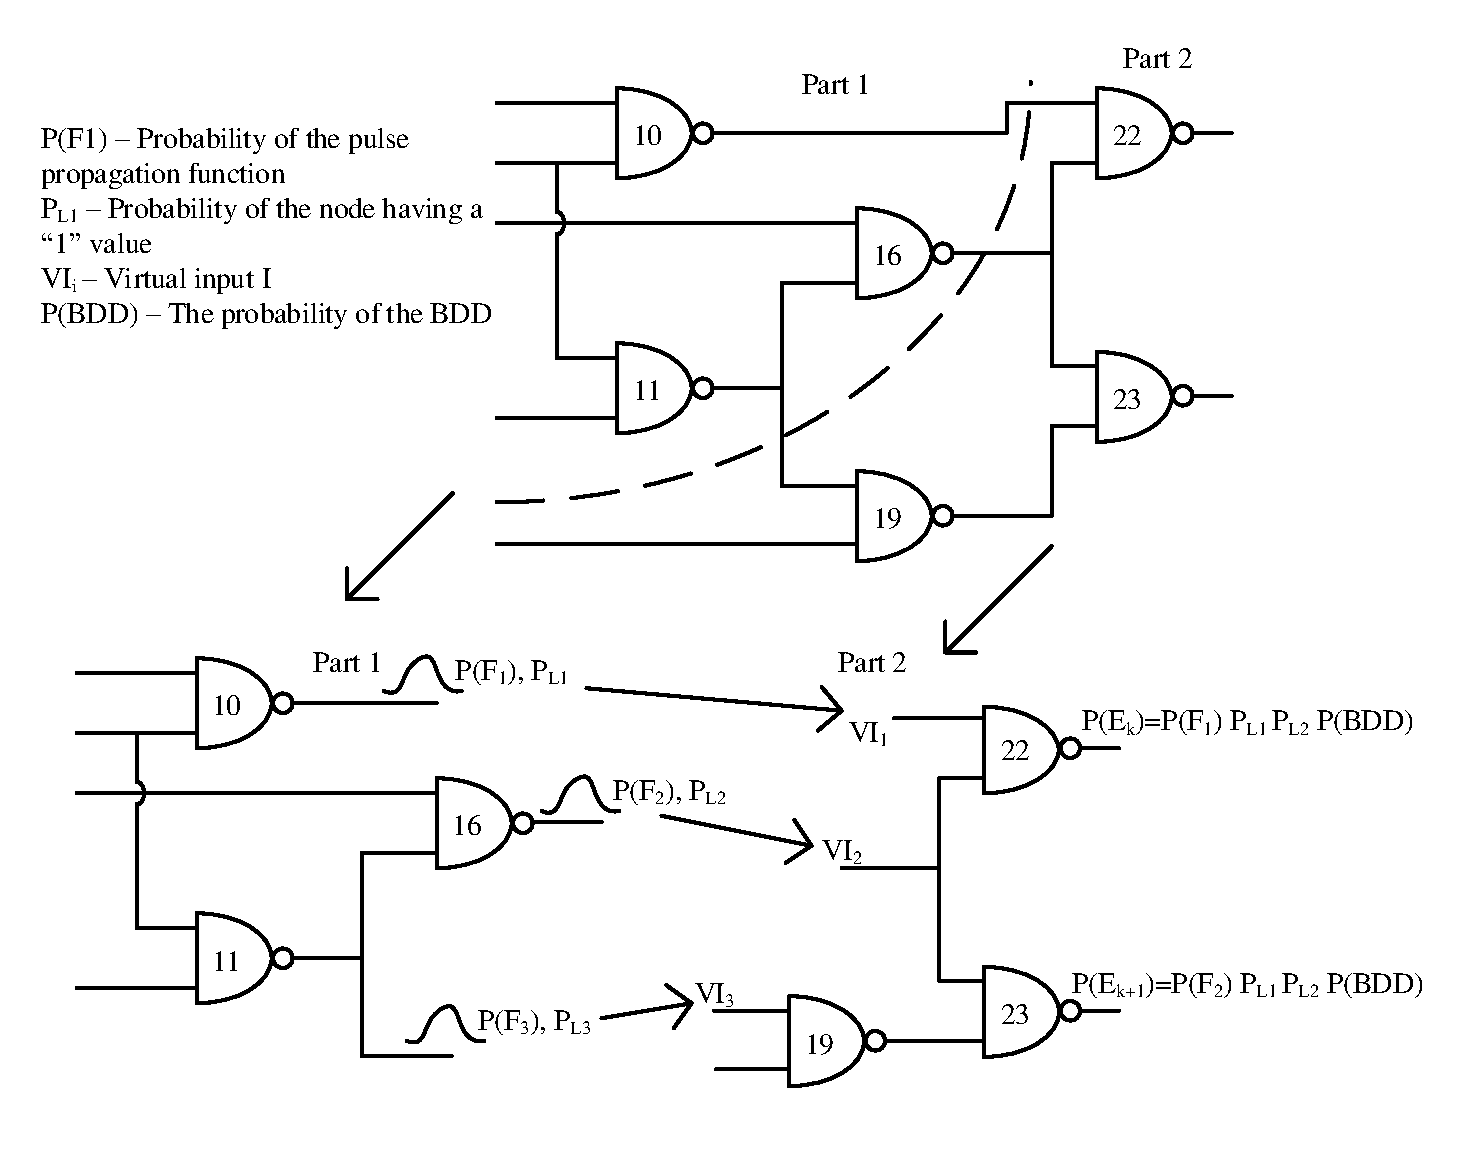
\includegraphics[width=\linewidth]{Figures/PartProp}
	%where an .eps filename suffix will be assumed under latex, 
	%and a .pdf suffix will be assumed for pdflatex; or what has been declared
	%via \DeclareGraphicsExtensions.
	\caption{An example on c17 showing how the pulses are propagated between partitions.}
	\label{PART_PROP}
\end{figure}

An issue that was found through numerous simulations using this method is that partitioning limits the inputs considered by a BDD function. In many cases, without partitioning, calculation of the BDD would result in a false value thus removing the pulse. However, because the functions are simplified in partitioning, they may not evaluate to false for these cases thus allowing the pulse to propagate. This, in effect, substantially reduces the number of pulses that are attenuated which can offset any improvement increases gained through partitioning. To solve this issue, it was found that setting a minimum probability threshold ($P_{thr}$) in which only pulses with a probability greater than this number are considered substantially saved simulation time with a slight increase in estimation error.

Once each individual pulse is propagated, a routine searches the input pulses and organizes them into a hash table based on their event number. For each event $E_k$, the pulses are checked for overlap. If the pulses do overlap, they are treated as convergent pulses and are considered as previously discussed. One issue that arises during this step is that there may be many possible cases in which the pulses overlap. For example, there may be 2, 3 or more concurrent overlapping pulses. In this work, to reduce the simulation time, only two pulses are considered. While the electrical masking model can accurately consider the effects of 3 or more convergent pulses, it is assumed that the likelihood of the pulses propagating is low.

Lastly, when the simulator processes a primary or partition output, the BDD functions for each pulse are solved to determine the probability. If the probability is solved on a primary output, the MES is determined as discussed in \ref{ch3:prelim}. An overview of the whole simulation flow is given in Algorithm \ref{alg:fastmet}.

\begin{algorithm}
	\caption{FAST\_MET} \label{alg:fastmet}
	\begin{algorithmic} [1]
		\STATE Set Process Parameters
		\STATE Parse Netlist
		\STATE Organize Circuit Topologically
		\STATE Parse Circuit Into $k$ Parts
		\FOR{Each Partition}
			\STATE Extract Partition
			\STATE Set Virtual Inputs
			\FOR{Each Gate} 	
				\STATE Generate Pulse
				\STATE Generate Logic Function
				\STATE Propagate Pulse
				\STATE Calculate Convergence
				\IF{Primary Output}
					\STATE Calculate $P_{L,i}$
				\ELSIF{Edge of Partition}
					\STATE Solve BDD Probability
				\ENDIF
			\ENDFOR
		\ENDFOR		
	\end{algorithmic}
\end{algorithm}

\begin{algorithm}
	\caption{Generate Pulse} 
	\begin{algorithmic} [1]
		\STATE F = Calculate Generation Function
		\IF{F != false}
			\STATE Calculate Pulse Shape
			\STATE Add To Pulse List
		\ENDIF		
	\end{algorithmic}
\end{algorithm}

\begin{algorithm}
	\caption{Propagate Pulse} 
	\begin{algorithmic} [1]
			\STATE $F_{log}$ = Logic Function
			\STATE $F_{sens}$ = Sensitization Function
			\FOR {Each Input $i$}
				\STATE $F_{sens}$ = $F_{log}$(i) $\land$ $F_{sens}$
			\ENDFOR		
			\IF{($F_{sens}$ != false) $\land$ (Solve BDD($F_{sens}$) $>$ $P_{thr}$)}
				\STATE Calculate Pulse Shape
				\STATE Add To Pulse List
			\ENDIF
	\end{algorithmic}
\end{algorithm}

\begin{algorithm}
	\caption{Calculate Convergence} 
	\begin{algorithmic} [1]
		\STATE Load Hash Table For Each Event
		\FOR {Each Event}
			\STATE I = Check For Overlap
			\IF {I == true}
				\STATE F = Calculate Convergence Function
				\IF {(F != false) $\land$ (Solve BDD(F) $>$ $P_{thr}$)}
					\STATE Calculate Pulse Shape
					\STATE Add To Pulse List
				\ENDIF
			\ENDIF
		\ENDFOR	
	\end{algorithmic}
\end{algorithm}
	
\section{Results} \label{ch3:results}

The FAST\_MET simulator was test on the ISCAS 85 combinational benchmark circuits. FAST\_MET was implemented in C++ on a machine with a quad core i7 and 16GB of RAM. The transistor look-up tables were characterized in HSPICE using the 32 nm Predictive Technology Model (PTM) \cite{PTM} where $V_{dd}$ was set to 1.05V. The unit gate capacitance was set to a constant capacitance of 2 fF to simulate the loading effects of the gates and interconnects. To calculate the MES, a single pulse with an energy of 15 fC was applied to each gate using equation \ref{qeq} with $\tau$ being set to $32x10^{-15}$. It was assumed that each output is connected to a flip-flop implemented in the same process library with a setup time ($t_{setup}$) of 22 ps and a hold time ($t_{hold}$) of -7 ps in accordance to \cite{Nunes2013}. For all simulations, the probability of MET was set to 10\% and the error threshold for simulation $P_{thr}$ was set to 0.025 when partitioning was used. When an MET occured, it was injected to a neighboring gate based on the netlist.

First, the accuracy of FAST\_MET without partitioning is compared to Monte Carlo simulation on c17 and c880 to ensure that the probabilistic functions provided here exactly compute the logical masking effect. To ensure that both simulators use the same pulses, the pulse injection routine in FAST\_MET was moved to before the main loop. Larger circuits were not tested since they lead to long simulation times and lead to memory blow up for FAST\_MET without the use of partitioning. As can be observed in the Table \ref{table:MCvFAST}, FAST\_MET provides exact estimation of the output error with an over 5x speedup.

\begin{table}[ht]
	\begin{center}
		\caption{Comparision of FAST\_MET vs Monte Carlo}
		\label{table:MCvFAST}
		\begin{tabular}{|c|c|c|c|}
			\hline
			Circuit& Simulator & MES & Run Time\\ 
			\hline
			c17 & Monte Carlo & $3.92x10^{-4}$ & 0.429\\
			\hline
			c880 & Monte Carlo & $4.15x10^{-4}$ & 9110.35\\
			\hline
			c17 & FAST\_MET & $3.92x10^{-4}$ & 0.0974\\
			\hline
			c880 & FAST\_MET & $4.15x10^{-4}$ & 1909.37\\
			\hline
		\end{tabular}
	\end{center}
\end{table}

The FAST\_MET simulator can provide an additional speedup through the use of partitioning. Table \ref{table:restable} provides the MES and the simulation time for various ISCAS 85 circuits while changing the partition size. According to the results, it shows that partitioning can provide an upward of 20X reduction in simulation time at a cost of accuracy compared to not using partitioning. Based off the results, it is shown that increasing the number of partitions follows the law of diminishing returns. For example in c880, the use of two partitions reduces the simulation time by 13X while the use of four partitions reduces the simulation time by 18X. While this is still a large decrease in simulation time, the error is increased by 4X. Additionally, it can be seen that in c17 the use of partitioning actually increases the simulation time. This is due to the time to simulate the circuit is less than the overhead incurred by the partitioning algorithm.

As observed by the results, it is necessary to determine the proper partition size to ensure an optimal trade-off between error and simulation time. For the current implementation, each partition was balanced based on the number of fan-in nodes to the gates. This is based on the assumption that gates with more fan-in nodes have a higher computational complexity due to more convergence cases and larger BDD sizes. To provide some direction on the ideal partition size, the average number of fan-in nodes among all partitions were counted and provided in Table \ref{table:restable}. For circuits c880 and c1355, the optimal trade-off between the error and simulation time was at a partition size of three hundred fan-in pins. On c1355, for example, the error between the MES for one partition (ideal) and the partitioned circuit for two and four partitions is $0.42x10^{-5}$ and $0.47x10^{-5}$ respectively. While the difference in error is very small, the simulation time is halved when four partitions are used. 

\begin{table}[ht]
	\begin{center}
		\caption{FAST\_MET Performance vs Number of Partitions}
		\label{table:restable}
		\begin{tabular}{|c|c|c|c|c|}
			\hline
			Circuit& Parts & MES & Run Time & Partition Size\\ 
			\hline
			c17 & 1 & $3.92x10^{-4}$ & 0.0974 & 12\\
			\hline
			c17 & 2 & $3.83x10^{-4}$ & 0.1377 & 6\\
			\hline
			c880 & 1 & $4.15x10^{-4}$ & 1909.37 & 729\\
			\hline
			c880 & 2 & $3.13x10^{-4}$ & 139.54 & 350\\
			\hline
			c880 & 4 & $8.37x10^{-4}$ & 107.72 & 180\\
			\hline
			c1355 & 1 & $2.38x10^{-4}$ & 3685.00 & 1064\\
			\hline
			c1355 & 2 & $1.96x10^{-4}$ & 459.00 & 536\\
			\hline
			c1355 & 4 & $2.85x10^{-4}$ & 242.60 & 270\\
			\hline
			c1355 & 8 & $3.67x10^{-4}$ & 167.961 & 135\\
			\hline
		\end{tabular}
	\end{center}
\end{table}

\section{Conclusion}
In this chapter, the FAST\_MET simulator is proposed. First, probabilistic equations were provided which allow for accurate consideration of all propagation effects. These equations were then represented as BDDs and used to determine the logical masking effect. In the results it was shown that the tool provides a good trade-off between simulation time and accuracy due to the use of partitioning and an accurate masking model. Additionally, it is shown that the number of partitions reduces the simulation time up 18x compared to not using partitioning and 90x compared to Monte Carlo simulation.

An open question that may occur is the consideration or process variations. In a realistic case, the transistor parameters given in the standard cells may vary considerably. For this reason, it is prudent to simulate circuits in which the gate process parameters vary by some amount. The electrical masking model proposed in this dissertation is able to consider process variations by characterizing look up tables for transistors that have differing parameters. Base of this, it is recommended to characterize at least 3 transistors look up tables, one with the lowest possible width, one with the highest width and one with an ideal value. Using these tables, multiple copies of the circuit can be created in which gates build randomly with the different tables are injected. For each circuit copied, the SER can be computed and analyzed.